\chapter{El caso finito}
\noindent
Debido a que $\vec{p} > \vec{0}$, resulta valioso mencionar que el problema
(\ref{theory:formulation}) es una instancia particular del famoso Problema de la Mochila
\begin{subequations}
	\label{knapsack-formulation}
	\begin{align}
		\max_{\vec{x} \in \Z^n} \quad
			& \vec{u}^T\vec{x}, \\
		\text{s.a.} \quad
			& \vec{w}^T\vec{x} \leq c, \\
			& \vec{x} \geq \vec{0},
	\end{align}
\end{subequations}
donde los vectores positivos $\vec{u}, \vec{w} \in \Z^n$ son conocidos como vector de útiles y
vector de pesos, respectivamente. Puesto que no acotamos $\vec{x}$, el problema recibe el nombre de
Problema de la Mochila no Acotado. Pero también como $\vec{u} = \vec{w}$, el problema
también puede ser considerado como un Problema de la Suma de Conjuntos no Acotado. En nuestro análisis
de resultados comparamos los tiempos de terminación de nuestro algoritmo con los de Ramificación y
Acotamiento, \texttt{MTU2} (\cite{martello}), y una formulación alternativa de programación dinámica.

\section{Análisis de capas enteras}
\noindent
De acuerdo al Teorema \ref{theory:th:feasibility}, el número de puntos factibles sobre la
$k$-ésima capa entera es finito y, por lo tanto, puede ser cero. No obstante, al igual que en la
sección anterior, somos capaces de caracterizar todos los puntos enteros que se encuentran en
cualquier capa entera. Consecuentemente, si determinamos que no hay ningún punto factible en la
$k$-ésima capa entera, descendemos a la $(k -1)$-ésima capa entera y realizamos el mismo
análisis.

En la primera parte de esta sección determinamos una cota superior para el número de capas enteras
que visitamos y analizamos el comportamiento a medida que el presupuesto $u$ aumenta. En la segunda
parte de esta sección mostramos que si el presupuesto $u$ es suficientemente grande, entonces la
solución de (\ref{theory:formulation}) sí se encuentra sobre la $\eta$-ésima capa entera. Este
resultado es análogo al caso infinito del Teorema \ref{theory:th:feasibility}. Finalmente, en la
tercera parte de esta sección discutimos brevemente sobre la complejidad algorítmica de encontrar
la solución.

\begin{lemma}
	Sea
	\begin{equation}
		\label{eq:last-index}
		i^* \coloneq \argmax \left\lbrace \frac{1}{\vec{q}_1}, \ldots, \frac{1}{\vec{q}_n} \right\rbrace,
	\end{equation}
	y definamos
	\begin{equation}
		\label{eq:tau}
		\tau \coloneq \left\lfloor \left\lfloor \frac{u}{\vec{q}_{i^*}} \right\rfloor
			\frac{\vec{q}_{i^*}}{m} \right\rfloor.
	\end{equation}
	Entonces la solución del problema (\ref{theory:formulation}) se encuentra en una capa entera
	parametrizada por $k \in \lbrace \eta, \eta - 1, \ldots, \tau \rbrace$.
\end{lemma}
\begin{proof}
	Consideremos el vector
	\begin{equation*}
		\vec{v} \coloneq \left\lfloor \frac{u}{\vec{q}_{i^*}} \right\rfloor \vec{e}_{i^*},
	\end{equation*}
	y observemos que $\vec{v} \geq \vec{0}$, pues $\vec{q} > \vec{0}$ y supusimos que el problema
	(\ref{theory:formulation}) es factible, por lo que $u \geq 0$. Así también, tenemos
	\begin{equation*}
		\vec{q}^T\vec{v} = \left\lfloor \frac{u}{\vec{q}_{i^*}} \right\rfloor \vec{q}_{i^*}
		\leq \frac{u}{\vec{q}_{i^*}}\vec{q}_{i^*} = u,
	\end{equation*}
	y entonces $\vec{v}$ es factible. De aquí se sigue que este vector provee una cota inferior para
	el problema (\ref{theory:formulation}). Así pues, todo vector $\vec{x}$ candidato a ser el
	óptimo del problema satisface
	\begin{equation*}
		\vec{q}^T\vec{x} = \frac{\vec{p}^T\vec{x}}{m} \geq \left\lfloor \frac{u}{\vec{q}_{i^*}}
		\right\rfloor \frac{\vec{q}_{i^*}}{m}.
	\end{equation*}
	Nos interesa calcular el número entero $\tau$ más pequeño tal que todo punto sobre la capa
	entera $H_{\vec{q}, k\norm{\vec{q}}^{-2}}$ con $k \in \lbrace \tau, \tau + 1, \ldots \rbrace$
	satisfaga esta desigualdad. Del Lema \ref{phase-1:lemma:layer}, toda $k$ debe satisfacer
	\begin{equation*}
		k\norm{\vec{q}}^{-2} = \frac{\vec{q}^T\vec{x}}{\norm{\vec{q}}^2} \geq
		\left\lfloor \frac{u}{\vec{q}_{i^*}} \right\rfloor \frac{\vec{q}_{i^*}}{m}
		\frac{1}{\norm{\vec{q}}^2},
	\end{equation*}
	y por lo tanto
	\begin{equation*}
		\tau =
		\left\lfloor \left\lfloor \frac{u}{\vec{q}_{i^*}} \right\rfloor \frac{\vec{q}_{i^*}}{m}
			\right\rfloor.
	\end{equation*}
	Finalmente, recordemos que $k$ es la primera capa en satisfacer la restricción presupuestaria.
	Por lo tanto, el óptimo del problema (\ref{theory:formulation}) se encuentra en una capa
	parametrizada por $k \in \lbrace \eta, \eta - 1, \ldots, \tau \rbrace$.
\end{proof}

\begin{observation}
	Siempre se cumple que $\tau \leq k$. En efecto,
	\begin{equation*}
		\left\lfloor \frac{u}{\vec{q}_{i^*}} \right\rfloor \vec{q}_{i^*}
		\leq \frac{u}{\vec{q}_{i^*}} \vec{q}_{i^*} = u,
	\end{equation*}
	como $m > 0$, tenemos
	\begin{equation*}
		\left\lfloor \frac{u}{\vec{q}_{i^*}} \right\rfloor \frac{\vec{q}_{i^*}}{m}
		\leq \frac{u}{m}.
	\end{equation*}
	Aplicando la función piso a ambos lados de la desigualdad encontramos que $\tau \leq k$.
\end{observation}
Sea $k \in \lbrace \eta, \eta - 1, \ldots, \tau \rbrace$. Sabemos de la sección de Fundamentos en el
primer capítulo que deseamos resolver la ecuación lineal diofantina
\begin{equation*}
	\vec{q}^T\vec{x} = \vec{q}_1\vec{x}_1 + \vec{q}_2\vec{x}_2 + \cdots + \vec{q}_n\vec{x}_n = k.
\end{equation*}
Implementamos la misma estrategia para plantear una formulación recursiva,
\begin{equation*}
	\frac{q_1}{g_1}\vec{x}_1 + g_2\omega_2 = \omega_1.
\end{equation*}
No obstante, en este caso podemos interpretar $\omega_2$ de tal manera que obtengamos más
información. Así como $\omega_1 \coloneq k$  es el presupuesto disponible en un inicio, $\omega_2$
es el presupuesto disponible después de utilizar parte de él para adquirir $\vec{x}_1 \geq 0$ unidades.
Por lo tanto, es posible agregar la restricción $\omega_2 \geq 0$. Similarmente, en el $i$-ésimo
paso de la formulación recursiva, somos capaces de agregar la restricción de que el presupuesto
restante $\omega_{i + 1}$ sea no negativo. Combinando esto con la no negatividad de $\vec{x}_i$, obtenemos
de (\ref{eq:recurrence}),
\begin{equation}
	\label{phase-1:finite:eq:param-bounds}
	\left\lceil -\frac{\omega_ix_i'}{g_{i+1}} \right\rceil
	\leq
	\vec{t}_i
	\leq
	\left\lfloor \frac{\omega_i\omega_{i+1}'}{\vec{q}_i} \prod_{j=1}^{i}g_j \right\rceil.
\end{equation}
para todo $i \in \lbrace 1, \ldots, n - 2\rbrace$. Después, como $0 < \vec{q}_{n - 1}, \vec{q}_n$, se sigue de
(\ref{eq:last-solution}),
\begin{equation}
	\label{phase-1:finite:eq:param-bounds-last}
	\left\lceil -\frac{\omega_{n-1}x_{n-1}'}{\vec{q}_n} \cdot \prod_{j=1}^{n-2}g_j \right\rceil
	\leq
	\vec{t}_{n - 1}
	\leq
	\left\lfloor \frac{\omega_{n-1}x_{n}'}{\vec{q}_{n-1}} \cdot \prod_{j=1}^{n-2}g_j \right\rfloor.
\end{equation}

Consecuentemente, el número de elecciones que podemos hacer para $\vec{t} \in \Z^{n-1}$ es finito.
Observemos que una elección de $\vec{t}_i$ modifica $\omega_{i+1}$ y por lo tanto también afecta el
intervalo de factibilidad de $\vec{t}_{i+1}$. Siguiendo con este razonamiento, encontramos que una
elección de $\vec{t}_i$ afecta los intervalos de factibilidad de $\vec{t}_{i+1}, \ldots,
\vec{t}_{n-1}$.

Es decir, a pesar de que el óptimo se encuentre sobre la capa entera $k$ que estamos analizando, la
elección de los primeros parámetros que realicemos puede afectar el tiempo de terminación de nuestro
algoritmo. Hay dos extremos en las posibles estrategias que podemos adoptar para realizar estas
elecciones. Para visualizarlo, tenemos que nuestro presupuesto actual $\omega_{i}$ determina el
siguiente presupuesto a partir de
\begin{equation*}
	\begin{cases}
		\vec{x}_i = \omega_ix_i' + g_{i+1}\vec{t}_i, \\
		\omega_{i+1} = \omega_i\omega_{i+1}' - \frac{\vec{q}_i}{\prod_{j=1}^{i}g_j}\vec{t}_i,
	\end{cases}
\end{equation*}
donde la primera ecuación indica cuántos elementos de $\vec{x}_i$ decidimos adquirir a partir del
presupuesto actual $\omega_i$.

El primer extremo está en buscar agotar todo nuestro presupuesto disponible en las primeras
elecciones de $\vec{x}_1, \vec{x}_2, \ldots, \vec{x}_i$. Es decir, adquirimos la mayor cantidad que
podamos de los primeros productos. Bajo esta perspectiva, es razonable imponer un orden en $\vec{q}$
de manera que
\begin{equation*}
	\vec{q}_1 \geq \vec{q}_2 \geq \cdots \geq \vec{q}_n,
\end{equation*}
por lo que primero adquirimos los artículos más caros. En este caso diremos que $\vec{q}$ está en
orden descendente. Si adoptamos esta estrategia es porque suponemos que el óptimo se concentra en
una vecindad de los primeros $i$ artículos. Es decir, si tenemos la creencia de que $\vec{x}_{i +
1}, \ldots, \vec{x}_n$ pueden ser aproximadamente cero.

% TODO: es mejor argumentar esto en la sección de análisis de resultados.
% De ser este el caso, entonces es razonable suponer que los tiempos de terminación de esta búsqueda
% son similares a los de Ramificación y Acotamiento. 

El segundo extremo es esencialmente lo opuesto. Esto no quiere decir que ahora ordenamos $\vec{q}$
de manera ascendente y escogemos las primera $\vec{t}_i$ lo más pequeñas posible\footnote{Si
	hiciéramos esto es porque creemos que $\vec{x}_1, \ldots, \vec{x}_i$ son aproximadamente cero,
	pero entonces podemos permutar estas entradas de manera que se encuentren hasta el final y
emplear la primera estrategia.}. Consiste en escoger $\vec{t}_i$ de manera que se encuentre en el
punto medio de sus cotas inferiores y superiores. Es decir, creemos que el óptimo se encuentra en
una vecindad del centro de masa de la $k$-ésima capa entera.

Observemos que, independientemente del caso, si una capa entera no contiene puntos factibles,
entonces ambas estrategias agotan todas las elecciones posibles de $\vec{t}_1, \ldots,
\vec{t}_{n-1}$. Por lo tanto, los tiempos de terminación de ambas estrategias son iguales para capas
enteras que no contienen puntos óptimos. La segunda estrategia, no obstante, es candidata ideal para
realizar una búsqueda binaria. Discutimos más sobre esto último en la sección de análisis de
resultados.

\begin{lemma}
	\label{lemma:layer-dist}
	Sean $q$ y $m$ enteros distintos de cero. Entonces la función $\Delta \colon \R \to \R$ dada por
	\begin{align*}
		\Delta(x) &\coloneq \left\lfloor \frac{x}{m} \right\rfloor - \left\lfloor \left\lfloor
		\frac{x}{q} \right\rfloor \frac{q}{m} \right\rfloor,
	\end{align*}
	es periódica con periodo $\lcm{q, m}$.
\end{lemma}
\begin{proof}
	Tenemos
	\begin{align*}
		\Delta(x + \lcm{q, m})
		&= \left\lfloor \frac{x}{m} + \frac{\lcm{q, m}}{m} \right\rfloor
		- \left\lfloor \left\lfloor \frac{x}{q} + \frac{\lcm{q,m}}{q} \right\rfloor \frac{q}{m}
			\right\rfloor,
	\end{align*}
	pero $q, m \mid \lcm{q, m}$, por lo que $\lcm{q,m}/m$ y $\lcm{q,m}/q$ son enteros. Por las
	propiedades de la función piso obtenemos los que queremos demostrar:
	\begin{align*}
		\Delta(x + \lcm{q,m})
		&=
		\left\lfloor \frac{x}{m} \right\rfloor + \frac{\lcm{q,m}}{m}
		- \left\lfloor \left\lfloor \frac{x}{q} \right\rfloor\frac{q}{m} + 
			\frac{\lcm{q,m}}{q}\cdot\frac{q}{m} \right\rfloor \\
		&= 
		\left\lfloor \frac{x}{m} \right\rfloor + \frac{\lcm{q,m}}{m}
		- \left\lfloor \left\lfloor \frac{x}{q} \right\rfloor\frac{q}{m}\right\rfloor
		- \frac{\lcm{q,m}}{m} \\
		&= 
		\left\lfloor \frac{x}{m} \right\rfloor
		- \left\lfloor \left\lfloor \frac{x}{q} \right\rfloor\frac{q}{m}\right\rfloor \\
		&= \Delta(x).
	\end{align*}
\end{proof}
\begin{definition}
	Sea $\vec{p} \in \R^n$ un vector esencialmente entero y sea $\vec{q} \in \Z^n$ su múltiplo
	coprimo. Consideremos los parámetros $\eta$ y $\tau$ (c.f. \ref{phase-1:lemma:eta},
	\ref{eq:tau}) como funciones del presupuesto $u$. Entonces decimos que la función $\Delta^*
	\colon \R \to \R$ dada por
	\begin{equation}
		\label{eq:dist-layers}
		\Delta^*(u) \coloneq \eta(u) - \tau(u)
	\end{equation}
	denota el número de capas enteras a revisar dado el presupuesto $u$.
\end{definition}

Si queremos aplicar el Lema \ref{lemma:layer-dist}, debemos reducir nuestra atención a vectores
$\vec{p} \in \Z^n$ distintos de cero. Esto se debe a que debemos asegurar que el múltiplo $m \neq 0$
sea entero\footnote{Es la creencia del autor que este resultado se puede generalizar para múltiplos
$m$ racionales, mas esto no agrega demasiado valor en lo que sigue de la tesis.}. Independientemente
del comportamiento periódico de $\Delta^*$, observemos que esta función varía significativamente en
ante cambios en $m$. Esto último implica que el número de capas enteras a revisar depende del número
de cifras decimales usadas para especificar $\vec{p}$.

\begin{example}
	\label{ex:decimals}
	Si tenemos $\vec{p} \coloneq (9.6, 7.2, 5.6)^T$, entonces $m = 0.8$ y por lo tanto el número de
	capas a revisar dado $u \coloneq 119$ es $\Delta^*(u) = 14$. En cambio, si tenemos $\vec{p} \coloneq
	(9.60, 7.28, 5.68)^T$, obtenemos $m = 0.08$, por lo que el número de capas a revisar dado $u$ es
	$\Delta^*(u) = 1499$. Es decir, si usamos una cifra decimal más, entonces $\Delta^*(u)$ se
	multiplica por 100, aproximadamente.
\end{example}

\begin{figure}[htbp]
  \centering

  \begin{minipage}[t]{0.48\textwidth}
    \centering
    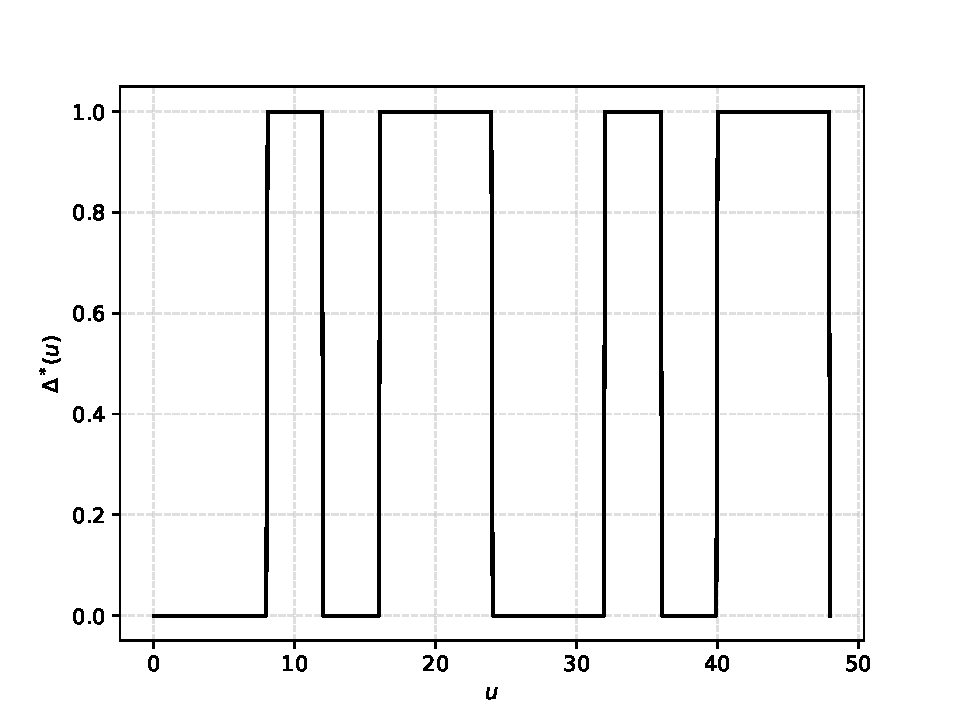
\includegraphics[width=\linewidth]{/home/tempdata/repos/thesis/static/delta8m12q.pdf}
  \end{minipage}
  \hfill
  \begin{minipage}[t]{0.48\textwidth}
    \centering
    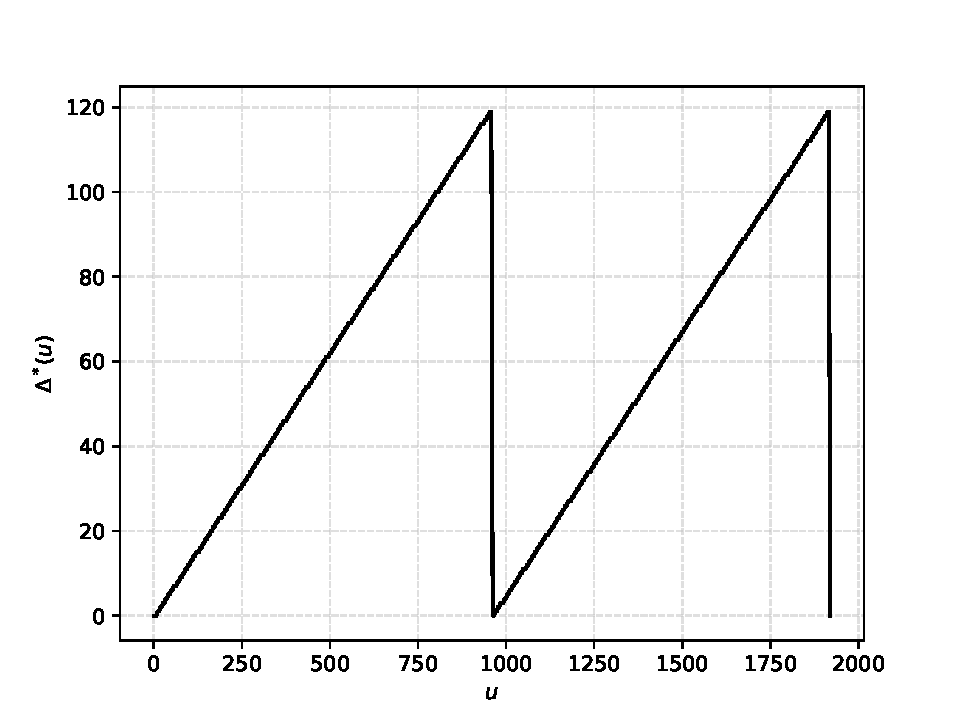
\includegraphics[width=\linewidth]{/home/tempdata/repos/thesis/static/delta008m960q.pdf}
  \end{minipage}

  \caption{Número de capas a revisar en función del presupuesto. \textit{Izquierda: }Para los
	  parámetros $m = 8$ y $\vec{q}_{i^*} = 12$ encontramos que hay un máximo de una capa a revisar.
	\textit{Derecha: } A medida que $m$ se vuelve fraccionario, las capas a revisar aumentan. En
		este caso tenemos $m = 0.08$ y $\vec{q}_{i^*} = 960$.}
\end{figure}

Observaremos en el análisis de resultados que el número de capas enteras que nuestro algoritmo
revisa en realidad disminuye a medida que aumenta el presupuesto $u$. Demostraremos a continuación
que para $u$ suficientemente grande, la solución al problema (\ref{theory:formulation}) se encuentra
en la $\eta$-ésima capa entera. Este resultado es análogo al caso infinito del Teorema
\ref{theory:th:feasibility}.

No obstante, necesitamos primero de un par de Definiciones y Lemas preliminares. Para motivar lo que
se encuentra a continuación mencionamos lo siguiente. Primero mostramos que existe un punto entero
en una vecindad fija de cada punto sobre la $k$-ésima capa entera. Luego, a medida que aumenta el
parámetro $k$, como la vecindad es fija, debe ser el caso que existe un punto entero no negativo en
la vecindad de cualquier otro punto no negativo.

Sea $H_{\vec{q}, k\norm{\vec{q}}^{-2}}$ una capa entera. Entonces definimos la bola cerrada sobre
esta capa entera con radio $r > 0$ y centro $\vec{x} \in H_{\vec{q}, k\norm{\vec{q}}^{-2}}$ como
\begin{equation}
	\label{eq:k-ball}
	B_r^{(k)}(\vec{x}) \coloneq \lbrace \vec{y} \in \R^n \colon \norm{\vec{y} - \vec{x}} \leq r
	\rbrace \cap H_{\vec{q}, k \norm{\vec{q}}^{-2}}.
\end{equation}
% TODO: mostrar una imagen con una bola.
\begin{lemma}
	\label{lemma:ball-cover}
	Existe $r > 0$ tal que la familia de bolas
	\begin{equation*}
		\left\lbrace B_r^{(k)}(\vec{x}) \colon \vec{x} \in H_{\vec{q}, k\norm{\vec{q}}^{-2}} \cap
			\Z^n \right\rbrace
	\end{equation*}
	es una cubierta de $H_{\vec{q}, k\norm{\vec{q}}^{-2}}$.
\end{lemma}
\begin{proof}
	Recordemos del Teorema (\ref{th:lattice}) que $\vec{x} \in H_{\vec{q}, k\norm{\vec{q}}^{-2}}
	\cap \Z^n$ si y solo si $\vec{x} = k\vec{\omega} + M\vec{t}$ para algún $\vec{t} \in \Z^{n-1}$.
	Así, tenemos
	\begin{equation*}
		\left\lbrace B_r^{(k)}(\vec{x}) \colon \vec{x} \in H_{\vec{q}, k\norm{\vec{q}}^{-2}} \cap
			\Z^n \right\rbrace
			=
		\left\lbrace B_r^{(k)}(k\vec{\omega} + M\vec{t}) \colon \vec{t} \in \Z^{n-1} \right\rbrace.
	\end{equation*}
	Por un lado, sabemos que $B_r^{(k)}(k\vec{\omega} + M\vec{t}) \subseteq H_{\vec{q}, k\norm{\vec{q}}^{-2}}$ para
	todo punto entero $\vec{t} \in \Z^{n-1}$. Luego, para cualquier $r > 0$ tenemos
	\begin{equation}
		\label{eq:ball-cover:1}
		\bigcup_{\vec{t} \in \Z^{n-1}}B_r^{(k)}(k\vec{\omega} + M\vec{t}) \subseteq
		H_{\vec{q}, k\norm{\vec{q}}^{-2}}.
	\end{equation}
	Ahora bien, sea $\vec{y}$ un punto sobre la $k$-ésima capa entera. Como las columnas de $M$ son
	linealmente independientes, existe $\vec{t} \in \R^{n-1}$ tal que
	\begin{equation*}
		\vec{y} = k\vec{\omega} + M\vec{t}.
	\end{equation*}
	Sea $\lfloor \vec{t} \rceil \in \Z^{n-1}$ el vector resultante de redondear cada entrada de
	$\vec{t}$ al entero más cercano. Luego, $\vec{t} = \lfloor \vec{t} \rfloor + \vec{\delta}$,
	donde $\vec{\delta} \in \R^{n-1}$ satisface $\norm{\vec{\delta}}_{\infty} \leq 0.5$. Definamos
	\begin{equation*}
		\vec{x} \coloneq k\vec{\omega} + M\lfloor \vec{t} \rceil \in \Z^{n-1},
	\end{equation*}
	de donde se sigue que
	\begin{align}
		\norm{\vec{y} - \vec{x}}_2^{2} 
		&= \norm{M\vec{\delta}}_{2}^{2} \nonumber \\
		&\leq \sum_{i=1}^{n-1}|\vec{\delta}_i|^2 \norm{M\vec{e}_i}_2^{2} \nonumber \\
		&\leq \frac{1}{4}\sum_{i=1}^{n-1} \norm{M\vec{e}_i}_2^{2} \label{eq:alt-M-bound} \\
		&= \frac{1}{4}\norm{M}_F^2, \nonumber
	\end{align}
	donde $\norm{M}_F$ denota la norma Frobenius de $M$. Por lo tanto, si definimos
	\begin{equation}
		\label{eq:radius}
		r \coloneq \frac{1}{2}\norm{M}_F,
	\end{equation}
	entonces para todo $\vec{y} \in H_{\vec{q}, k\norm{\vec{q}}^{-2}}$, existe $\vec{x} \in \Z^n$
	sobre esa misma capa entera tal que $\vec{y} \in B_r^{(k)}(\vec{x})$. Por lo tanto,
	\begin{equation}
		\label{eq:ball-cover:2}
		H_{\vec{q}, k\norm{\vec{q}}^{-2}} \subseteq
		\bigcup_{\vec{t} \in \Z^{n-1}}B_r^{(k)}(k\vec{\omega} + M\vec{t}).
	\end{equation}
	Juntando esto con (\ref{eq:ball-cover:1}) obtenemos lo que queríamos demostrar.
\end{proof}

Ahora bien, denotemos por $\vec{u}_i$ las intersecciones que tiene la capa entera $H_{\vec{q},
k\norm{\vec{q}}^{-2}}$ con cada uno de los ejes. Es decir,
\begin{equation}
	\label{eq:generators}
	\vec{u}_i \coloneq \frac{k}{\vec{q}_i}\vec{e}_i,
\end{equation}
y consideremos el símplice $\sigma$ generado por estos vectores:
\begin{equation*}
	\sigma \coloneq \left\lbrace \theta_1\vec{u}_1 + \cdots \theta_n\vec{u}_n \colon
		\sum_{i=1}^{n}\theta_i = 1, \theta_i \geq 0 \right\rbrace.
\end{equation*}
No es difícil ver que todo punto $\vec{x} \in \R^n_{\geq \vec{0}}$ sobre la $k$-ésima capa entera
también es un elemento de este símplice $\sigma$ y viceversa.

Ahora bien, nos interesa determinar la existencia de un punto entero sobre $\sigma$. De esta manera,
tendríamos un punto entero no negativo que satisface la ecuación lineal diofantina
$\vec{q}^T\vec{x} = k$. Para lograr esto, definimos el baricentro del $\sigma$ y determinamos una
vecindad de este baricentro de manera que esté contenida en el símplice.

\begin{definition}
	Dado un símplice $\sigma$ generado por $\vec{u}_1, \ldots, \vec{u}_n$, definimos su baricentro o
	centro de masa $\est{\sigma}$ como
	\begin{equation*}
		\est{\sigma} \coloneq \frac{1}{n} \sum_{i=1}^{n}\vec{u}_i.
	\end{equation*}
\end{definition}
\begin{observation}
	El baricentro $\est{\sigma}$ es un elemento de $\sigma$. Esto se debe a que $\est{\sigma}$ es la
	combinación convexa de $\vec{u}_1, \ldots, \vec{u}_n$, donde $\theta_1 = \cdots = \theta_n =
	\frac{1}{n}$.
\end{observation}

\begin{definition}
	Sea $\sigma$ un símplice y consideremos su baricentro $\est{\sigma}$. Definamos
	\begin{equation}
		\label{eq:def:r-sigma}
		r_\sigma \coloneq \max \lbrace r > 0 \colon B_r^{(k)}(\est{\sigma})
		\subseteq \sigma \rbrace.
	\end{equation}
	Entonces decimos que $\mathcal{C}^{(k)} \coloneq
	B_{r_\sigma}^{(k)}(\est{\sigma})$ es la circunferencia inscrita en $\sigma$. A
	$r_\sigma$ le llamamos el radio de tal circunferencia.
\end{definition}

\begin{definition}
	Sea $\sigma$ un símplice. Al símplice $F_j$ generado por los vectores $\lbrace \vec{u}_i
	\rbrace_{i \neq j}$ lo llamamos la $j$-ésima faceta de $\sigma$.
\end{definition}
\begin{observation}
	Si $\sigma$ es generado por $n$ vectores, entonces tiene $\binom{n}{n-1} = n$ facetas, y cada
	una es generada por $n - 1$ vectores. También se cumple que la frontera del símplice es $F_1
	\cup \cdots \cup F_n$.
\end{observation}

De (\ref{eq:generators}) encontramos que el vector $\vec{u}_j$ es ortogonal a los vectores $\lbrace
\vec{u}_i \rbrace_{i \neq j}$, se sigue que su proyección sobre la capa entera $H_{\vec{q},
k\norm{\vec{q}}_2^{-2}}$ es el vector normal de la faceta $F_j$. Además, esta proyección apunta
hacia el interior del símplice $\sigma$. Ahora bien, como $\vec{q}$ es el vector normal a
$H_{\vec{q}, k\norm{\vec{q}}_2}$, encontramos que la proyección de $\vec{u}_j$ sobre esta capa
entera es
\begin{equation}
	\label{eq:normal-vector}
	\vec{\mu}_j \coloneq
	\vec{u}_j - \frac{\vec{q}^T\vec{u}_j}{\vec{q}^T\vec{q}}\vec{q}
	=
	\vec{u}_j - \frac{k}{\norm{\vec{q}}_2^2}\vec{q}.
\end{equation}
Denotemos por $\est{\mu}_j$ el vector $\vec{\mu}_j$ normalizado. Encontramos entonces que cada
faceta $F_j$ está contenida en el hiperplano afino
\begin{equation*}
	\lbrace \vec{x} \in \R^{n} \colon \est{\mu}_j^T\vec{x} = b_j \rbrace
	\cap H_{\vec{q}, k\norm{\vec{q}}_2^{-2}},
\end{equation*}
donde $b_j \coloneq \est{\mu}_j^T\vec{x}$ para algún $\vec{x} \in F_j$. Luego, como cada
vector normal $\est{\mu}_j$ apunta hacia el interior del símplice $\sigma$, se sigue que
podemos escribirlo como
\begin{equation*}
	\sigma = \bigcap_{j=1}^{n} \lbrace \vec{x} \in \R^{n} \colon \est{\mu}^T_j\vec{x} \geq b_j
	\rbrace \cap H_{\vec{q}, k\norm{\vec{q}}_2^{-2}}.
\end{equation*}
Esta caracterización de $\sigma$ nos permite demostrar el siguiente Lema.
\begin{lemma}
	\label{lemma:sigma-radius}
	El radio $r_\sigma$ de la circunferencia inscrita en $\sigma$ está dado por
	\begin{equation*}
		r_\sigma = \min_{1 \leq j \leq n} \lbrace d(\est{\sigma}, F_j) \rbrace,
	\end{equation*}
	donde $d(\est{\sigma}, F_j)$ denota la mínima distancia entre el baricentro
	$\est{\sigma}$ y la $j$-ésima faceta $F_j$ del símplice $\sigma$.
\end{lemma}
\begin{proof}
	Observemos que $\vec{u}_i$ con $i \neq j$ es un vector sobre el símplice $\sigma$. Luego, la
	distancia entre el baricentro y la $j$-ésima faceta es
	\begin{equation*}
		d(\est{\sigma}, F_j) = |\est{\mu}_j^T(\est{\sigma} - \vec{u}_i)|
		= \est{\mu}_j^T(\est{\sigma} - \vec{u}_i),
	\end{equation*}
	pues $\est{\sigma}$ es un elemento de $\sigma$ y $\est{\mu}_j$ apunta hacia adentro
	del símplice.

	Mostramos primero que si $r \leq \min_{1 \leq j \leq n} \lbrace d(\est{\sigma}, F_j) \rbrace$, entonces
	$B_r^{(k)}(\est{\sigma}) \subseteq \sigma$. Así pues, sea $\vec{x} \in
	B_r^{(k)}(\est{\sigma})$. Observemos que
	\begin{align*}
		\est{\mu}_j^T\vec{x} - b_j
		&=
		\est{\mu}_j^T(\vec{x} - \est{\sigma}) + \est{\mu}_j^T\est{\sigma} -
		b_j \\
		&= \est{\mu}_j^T(\vec{x} - \est{\sigma}) + d(\est{\sigma}, F_j).
	\end{align*}
	Por Cauchy-Schwartz tenemos
	\begin{equation*}
		\est{\mu}_j^T(\vec{x} - \est{\sigma}) \geq -\norm{\est{\mu}_j}_2\norm{\vec{x} -
		\est{\sigma}}_2 = -\norm{\vec{x} - \est{\sigma}}_2 \geq -r,
	\end{equation*}
	y por lo tanto,
	\begin{equation*}
		\est{\mu}_j^T\vec{x} - b_j \geq -r + d(\est{\sigma}, F_j) \geq 0,
	\end{equation*}
	pues $r \leq d(\est{\sigma}, F_j)$ para todo $j \in \lbrace 1, \ldots, n \rbrace$. Así,
	encontramos que, para todo $\vec{x} \in B_r^{(k)}(\est{\sigma})$,
	\begin{equation*}
		\vec{x} \in
		\bigcap_{j=1}^{n} \lbrace \vec{x} \in \R^{n-1} \colon \est{\mu}^T_j\vec{x} \geq b_j \rbrace
		\cap H_{\vec{q}, k\norm{\vec{q}}_2^{-2}} = \sigma,
	\end{equation*}
	y por lo tanto $B_r^{(k)}(\est{\sigma}) \subseteq \sigma$. A causa de
	(\ref{eq:def:r-sigma}) encontramos que $r_\sigma \geq \min_{1 \leq j \leq n} \lbrace
	d(\est{\sigma}, F_j) \rbrace$.

	Ahora bien, supongamos que $r > d(\est{\sigma}, F_j)$ para algún $j \in \lbrace 1, \ldots,
	n \rbrace$. Consideremos el punto $\vec{x} \in F_j$ que satisface $d(\est{\sigma}, F_j) =
	d(\est{\sigma}, \vec{x})$. Tal punto existe porque $F_j$ es cerrado. Luego,
	$\norm{\vec{\sigma} - \vec{x}}_2 < r$. Entonces existe $\varepsilon > 0$ tal que
	\begin{equation*}
		\norm{\est{\sigma} - (\vec{x} - \varepsilon\est{\mu}_j)}_2 \leq r,
	\end{equation*}
	lo que implica que $\vec{x} - \varepsilon\est{\mu}_j \in
	B_r^{(k)}(\est{\sigma})$. Sin embargo, tenemos
	\begin{equation*}
		\est{\mu}_j^T(\vec{x} - \varepsilon\est{\mu}_j) = b_j - \varepsilon\norm{\est{\mu}_j}_2^2 < b_j,
	\end{equation*}
	y entonces $\vec{x} - \varepsilon\est{\mu} \not\in \sigma$. De aquí se sigue que $r_\sigma
	\leq d(\est{\sigma}, F_j)$ para todo $j \in \lbrace 1, \ldots, n \rbrace$ y, por lo tanto,
	$r_\sigma \leq \min_{1 \leq j \leq n} \lbrace d(\est{\sigma}, F_j) \rbrace$.

	Concluimos, entonces, con
	\begin{equation*}
		r_\sigma = \min_{1 \leq j \leq n} \lbrace d(\est{\sigma}, F_j) \rbrace,
	\end{equation*}
	que es lo que queríamos demostrar.
\end{proof}

Buscamos expresar el radio $r_\sigma$ en función de $k$, por lo que debemos realizar un par de
cálculos. Retomemos de la demostración del Lema anterior que la distancia entre el baricentro y la
$j$-ésima faceta está dada por
\begin{equation*}
	d(\est{\sigma}, F_j) = \frac{{\vec{\mu}}_j^T(\est{\sigma} - \vec{\mu}_j)}{\norm{\vec{\mu}_j}_2}.
\end{equation*}
Realizando los cálculos, encontramos que
\begin{align*}
	\vec{\mu}_j^T(\est{\sigma} - \vec{u}_i)
	% &=
	% \left( \frac{k}{\vec{q}_j}\vec{e}_j - \frac{k}{\norm{\vec{q}}_2^2}\vec{q} \right)^T
	% \left( \frac{k}{n\vec{q}_1}, \ldots, \frac{k}{n\vec{q}_i} - \frac{k}{\vec{q}_i}, \ldots,
	% 		\frac{k}{n\vec{q}_n} \right) \\
	% &=
	% k^2
	% \left( \frac{1}{\vec{q}_j}\vec{e}_j - \frac{1}{\norm{\vec{q}}_2^2}\vec{q} \right)^T
	% \left( \frac{1}{n\vec{q}_1}, \ldots, \frac{1}{n\vec{q}_i} - \frac{1}{\vec{q}_i}, \ldots,
	% 		\frac{1}{n\vec{q}_n} \right) \\
	% &=
	% k^2
	% \left(\frac{1}{\vec{q}_j}\frac{1}{n\vec{q}_j} -
	% 	\frac{1}{\norm{\vec{q}}_2^2} \cdot
	% 	\left(\frac{1}{n} + \cdots + \frac{1}{n} - 1\right)
	% 	\right) \\
	&= \frac{k^2}{n\vec{q}_j^2},
\end{align*}
y también
\begin{equation*}
	\norm{\vec{\mu}_j}_2 = k \sqrt{\frac{1}{\vec{q}_j^2} - \frac{1}{\norm{\vec{q}}_2^2}}.
\end{equation*}
Sustituyendo valores, obtenemos
\begin{equation*}
	d(\est{\sigma}, F_j) = \frac{k}{n} \cdot
	\frac{1}{\vec{q}_j^2\sqrt{\vec{q}_j^{-2} - \norm{\vec{q}}_2^{-2}}}
	= \frac{k}{n} \cdot \frac{1}{Q_j},
\end{equation*}
donde definimos $Q_j$ pertinentemente. Finalmente, del Lema \ref{lemma:sigma-radius} encontramos que
el radio de la circunferencia inscrita en el símplice $\sigma$ está dado por
\begin{equation}
	\label{eq:sigma-radius}
	r_\sigma = \min_{1 \leq j \leq n} \lbrace d(\est{\sigma}, F_j) = \frac{k}{n} \cdot
	\frac{1}{\max_{1 \leq j \leq n} \lbrace Q_j \rbrace}
\end{equation}

\begin{theorem}
	Existe un punto entero sobre el símplice $\sigma$ para $k$ suficientemente grande.
\end{theorem}
\begin{proof}
	Consideremos $r$ definida en (\ref{eq:radius}). Por el Lema \ref{lemma:ball-cover} sabemos que
	existe un punto entero $\vec{x}$ en $B_r^{(k)}(\est{\sigma})$. Como la circunferencia
	$\mathcal{C}^{(k)}$ está inscrita en $\sigma$, basta mostrar que existe $k$
	suficientemente grande tal que $r \leq r_\sigma$, pues esto implicaría
	\begin{equation*}
		\vec{x} \in B_r^{(k)}(\est{\sigma}) \subseteq \mathcal{C}^{(k)} \subseteq \sigma.
	\end{equation*}
	De (\ref{eq:sigma-radius}) obtenemos que $r \leq r_\sigma$ si y solo si
	\begin{equation}
		\label{eq:eta-limit}
		k \geq \frac{n}{2}\norm{M}_F\max_{1 \leq j \leq n} \lbrace Q_j \rbrace,
	\end{equation}
	que es lo que queríamos demostrar.
\end{proof}
De manera inmediata obtenemos los siguientes Corolarios.
\begin{corollary}
	La ecuación lineal diofantina $\vec{q}^T\vec{x} = \eta$ tiene soluciones enteras no negativas para
	$\eta$ suficientemente grande.
\end{corollary}
\begin{corollary}
	El problema (\ref{theory:formulation}) se puede resolver a partir de una ecuación lineal
	diofantina para $u$ suficientemente grande.
\end{corollary}

Vale la pena hacer un par de observaciones. En primer lugar, de (\ref{eq:eta-limit}) parece que
podemos concluir que hay una dependencia lineal entre la dimensión $n$ y el lado derecho $k$. No
obstante, la norma $\norm{M}_F$ también depende de la dimensión. Para ser más explícitos con
respecto a esta dependencia, podemos rescatar de (\ref{eq:alt-M-bound}) la siguiente cota:
\begin{equation*}
	\frac{1}{4}\sum_{i=1}^{n-1}\norm{M\vec{e}_i}_2^2
	\leq
	\frac{n-1}{4}\max_{1 \leq j \leq n} \lbrace \norm{M\vec{e}_j}_2^2 \rbrace,
\end{equation*}
de donde obtendríamos
\begin{equation*}
	k \geq \frac{n\sqrt{n-1}}{2} \max_{1 \leq j \leq n} \lbrace \norm{M\vec{e}_j}_2 \rbrace \cdot
	\max_{1 \leq j \leq n} \lbrace Q_j \rbrace.
\end{equation*}
Esta cota, no obstante, es menos ajustada que la propuesta inicialmente.

En segundo lugar, el resultado que obtuvimos es más fuerte de lo que aparenta. Hemos encontrado una
cota inferior de manera que podamos asegurar la existencia de soluciones enteras en una vecindad del
baricentro $\est{\sigma}$. Este punto no es especial, en realidad podemos realizar el mismo
procedimiento enfocándonos en otros puntos del símplice $\sigma$ para asegurar soluciones en sus
respectivas vecindades. Entonces, dependiendo del punto, podemos obtener mejores o peores cotas para
$k$. El punto más interesante es aquel que provee la cota inferior más pequeña\footnote{
	El autor tiene razones para sospechar que este punto se encuentra en la intersección de todos
	los vectores normales a cada faceta $F_j$.
}.

En tercer lugar, la cota (\ref{eq:eta-limit}) provee, hasta donde llega el conocimiento del autor,
nuevas cotas superiores para los números de Frobenius. De manera resumida, dada una colección de
enteros $a_1, \ldots, a_n$ coprimos, el número de Frobenius es el entero $F$ más grande tal que $F$
no pueda ser expresado como una combinación lineal entera no negativa de $a_1, \ldots, a_n$. Un
estudio sobre cómo se compara esta colección de cotas con respecto a la literatura existente, si
bien interesante, queda fuera del propósito de esta tesis.

En cuarto lugar, cabe mencionar que eventualmente es suficiente con revisar la primera capa entera.
No hemos demostrado, empero, que el número de capas enteras a revisar eventualmente decrece en
cuanto $u$ aumenta. Observaremos en el análisis de resultados que hay un patrón periódico y
decreciente en cuanto al número de capas enteras revisadas. Demostrar que este comportamiento se
cumple es mucho más difícil y queda fuera del propósito de esta tesis.

\subsection{Complejidad algorítmica}
\noindent
Con respecto a la complejidad algorítmica de analizar capas enteras podemos decir lo siguiente.
Supongamos que deseamos encontrar todas las soluciones de (\ref{theory:formulation}). Definamos
\begin{equation}
	\label{phase-1:def:feasible-layer}
	P_k \coloneq H_{\vec{q}, k\norm{\vec{q}}^{-2}} \cap \Z_{\geq \vec{0}}^n
	=
	\lbrace \vec{x} \in \Z^n \vcentcolon \vec{q}^T\vec{x} = k, \vec{x} \geq \vec{0}
	\rbrace,
\end{equation}
y sea $T(n)$ el tiempo requerido para encontrar todos los puntos en $P_k$ o determinar que este
conjunto es vacío. Es razonable suponer que $T(n)$ es exponencial en $n$. En efecto, cada par
$(\vec{x}_i, \omega_{i + 1})$ genera un intervalo de factibilidad $[\vec{t}_i^{\min},
\vec{t}_i^{\max}]$. Este intervalo ciertamente depende de las elecciones previas de $\vec{t}_1, \ldots,
\vec{t}_{i - 1}$, aunque suprimimos esta dependencia en la notación para tener mayor claridad. Para
encontrar todos los puntos en $P_k$, el algoritmo recorre todas las posibilidades:
\begin{equation}
	\label{phase-1:complexity:bounds}
	\prod_{i=1}^{\kappa_1} \min_{\vec{t}_1, \ldots, \vec{t}_{i-1}} \lbrace \vec{t}_i^{\max} -
	\vec{t}_i^{\min} \rbrace
	\leq T(n) \leq
	\prod_{i=1}^{\kappa_2} \max_{\vec{t}_1, \ldots, \vec{t}_{i-1}} \lbrace \vec{t}_i^{\max} -
	\vec{t}_i^{\min} \rbrace,
\end{equation}
donde $1 \leq \kappa_1 \leq n$ es el entero más grande que asegura que  $\min_{\vec{t}_1, \ldots,
\vec{t}_{i - 1}}\lbrace \vec{t}_i^{\max} - \vec{t}_i^{\min} \rbrace$ sea positivo para todo $i \in
\lbrace 1, \ldots, \kappa_1 \rbrace$. Definimos $\kappa_2$ de manera análoga. Se cumple que
$\kappa_1 \leq \kappa_2$. Sean $\ell_{\min}, \ell_{\max}$ las longitudes del intervalo de
factibilidad más pequeño y del más grande en todos los niveles, respectivamente. Es decir, definimos
\begin{align}
	\ell_{\min} &\coloneq \min_{1 \leq i \leq \kappa_1} \left\lbrace \min_{\vec{t}_1, \ldots,
	\vec{t}_{i - 1}} \lbrace \vec{t}_i^{\max} - \vec{t}_i^{\min} \rbrace \right\rbrace,
	\\
			\ell_{\max} &\coloneq \max_{1 \leq i \leq \kappa_2} \left\lbrace \max_{\vec{t}_1,
			\ldots, \vec{t}_{i - 1}} \lbrace \vec{t}_i^{\max} - \vec{t}_i^{\max} \rbrace
		\right\rbrace.
\end{align}
Si $P_k$ es vacío, se sigue que no existe ningún intervalo factible en el nivel $n$, lo que implica
que $\kappa_2 < n$. En caso contrario, el algoritmo recorre hasta el último nivel, por lo que $\kappa_1
= \kappa_2 = n$. De (\ref{phase-1:complexity:bounds}), obtenemos
\begin{equation}
	\ell_{\min}^{n} \leq T(n) \leq \ell_{\max}^{n}.
\end{equation}
En el peor de los casos, nuestro algoritmo recorre todas las capas enteras parametrizadas por
$\lbrace k, k - 1, \ldots, \tau\rbrace$. Se sigue que
\begin{align}
	\label{phase-1:time}
	\text{Tiempo de ejecución}
	= \mathcal{O}((k - \tau) \cdot T(n))
	= \mathcal{O}(c^{n}),
\end{align}
para alguna $c > 1$.

Ahora bien, este razonamiento aplica a la modificación de nuestro objetivo en donde decidimos buscar
todas las soluciones posibles. En realidad solo nos interesa encontrar un punto óptimo, por lo que
podemos concluir que una cota superior para la complejidad de nuestro algoritmo es
(\ref{phase-1:time}). Asímismo, en la práctica encontramos que la diferencia $k - \tau$ es crucial
para determinar cuántas capas enteras recorre nuestro algoritmo en el peor de los casos.

Hemos mostrado anteriormente que para $u$ suficientemente grande es suficiente con recorrer una
capa. En caso de que $u$ no sea suficientemente grande, observaremos en el análisis de resultados
cómo se distribuye el número de capas enteras que en realidad se visitan.

\section{Análisis de resultados}

\section{Aplicaciones}
